\documentclass{article}
\usepackage{amsmath,amsfonts,amsthm,amssymb}
\usepackage{setspace}
\usepackage{fancyhdr}
\usepackage{lastpage}
\usepackage{extramarks}
\usepackage{chngpage}
\usepackage{soul,color}
\usepackage{graphicx,float,wrapfig}
\usepackage{CJK}
\usepackage{algorithm}  
\usepackage{algpseudocode} 
\usepackage{enumerate}
\usepackage{longtable}
\usepackage{listings}
\usepackage{color}
\usepackage{extarrows}
\usepackage{subfigure}
\usepackage{framed}
\usepackage{multirow}
\usepackage{makecell}

\usepackage{natbib}
\renewcommand{\bibname}{References}
\renewcommand{\bibsection}{\subsubsection*{\bibname}}

\newcommand{\Class}{Deep Learning}
\newcommand{\ClassInstructor}{Yi Wu}

% Homework Specific Information. Change it to your own
\newcommand{\Title}{Homework 4}
\newcommand{\DueDate}{May 14, 2021}
\newcommand{\StudentName}{Runlong Zhou}
\newcommand{\StudentClass}{YaoClass 82}
\newcommand{\StudentNumber}{2018011309}

% In case you need to adjust margins:
\topmargin=-0.45in      %
\evensidemargin=0in     %
\oddsidemargin=0in      %
\textwidth=6.5in        %
\textheight=9.0in       %
\headsep=0.25in         %

% Setup the header and footer
\pagestyle{fancy}                                                       %
\lhead{\StudentName}                                                 %
\chead{\Title}  %
\rhead{\firstxmark}                                                     %
\lfoot{\lastxmark}                                                      %
\cfoot{}                                                                %
\rfoot{Page\ \thepage\ of\ \protect\pageref{LastPage}}                          %
\renewcommand\headrulewidth{0.4pt}                                      %
\renewcommand\footrulewidth{0.4pt}                                      %

%%%%%%%%%%%%%%%%%%%%%%%%%%%%%%%%%%%%%%%%%%%%%%%%%%%%%%%%%%%%%
% Some tools
\newcommand{\enterProblemHeader}[1]{\nobreak\extramarks{#1}{#1 continued on next page\ldots}\nobreak%
                                    \nobreak\extramarks{#1 (continued)}{#1 continued on next page\ldots}\nobreak}%
\newcommand{\exitProblemHeader}[1]{\nobreak\extramarks{#1 (continued)}{#1 continued on next page\ldots}\nobreak%
                                   \nobreak\extramarks{#1}{}\nobreak}%

\newcommand{\homeworkProblemName}{}%
\newcounter{homeworkProblemCounter}%
\newenvironment{homeworkProblem}[1][Problem \arabic{homeworkProblemCounter}]%
  {\stepcounter{homeworkProblemCounter}%
   \renewcommand{\homeworkProblemName}{#1}%
   \section*{\homeworkProblemName}%
   \enterProblemHeader{\homeworkProblemName}}%
  {\exitProblemHeader{\homeworkProblemName}}%

\newcommand{\homeworkSectionName}{}%
\newlength{\homeworkSectionLabelLength}{}%
\newenvironment{homeworkSection}[1]%
  {% We put this space here to make sure we're not connected to the above.

   \renewcommand{\homeworkSectionName}{#1}%
   \settowidth{\homeworkSectionLabelLength}{\homeworkSectionName}%
   \addtolength{\homeworkSectionLabelLength}{0.25in}%
   \changetext{}{-\homeworkSectionLabelLength}{}{}{}%
   \subsection*{\homeworkSectionName}%
   \enterProblemHeader{\homeworkProblemName\ [\homeworkSectionName]}}%
  {\enterProblemHeader{\homeworkProblemName}%

   % We put the blank space above in order to make sure this margin
   % change doesn't happen too soon.
   \changetext{}{+\homeworkSectionLabelLength}{}{}{}}%

\newcommand{\Answer}{\textbf{Answer:} }
\newcommand{\Acknowledgement}[1]{\ \\{\bf Acknowledgement:} #1}

%%%%%%%%%%%%%%%%%%%%%%%%%%%%%%%%%%%%%%%%%%%%%%%%%%%%%%%%%%%%%


%%%%%%%%%%%%%%%%%%%%%%%%%%%%%%%%%%%%%%%%%%%%%%%%%%%%%%%%%%%%%
% Make title
\title{\textmd{\bf \Class: \Title}\\{\large Instructed by \textit{\ClassInstructor}}\\\normalsize\vspace{0.1in}\small{Due\ on\ \DueDate}}
\date{}
\author{\textbf{\StudentName}\ \ \StudentClass\ \ \StudentNumber}
%%%%%%%%%%%%%%%%%%%%%%%%%%%%%%%%%%%%%%%%%%%%%%%%%%%%%%%%%%%%%


%%%%%%%%%%%%%%%%%%%%%%%%%%%%%%%%%%%%%%%%%%%%%%%%%%%%%%%%%%%%%
% Listing Settings
\definecolor{mygreen}{rgb}{0,0.6,0}
\definecolor{mygray}{rgb}{0.5,0.5,0.5}
\definecolor{mymauve}{rgb}{0.58,0,0.82}

\definecolor{shadecolor}{rgb}{0.92,0.92,0.92}

\lstset{
  aboveskip=1em,                   % above skip space
  backgroundcolor=\color[rgb]{0.9,0.9,0.9},
                                   % choose the background color; you must add \usepackage{color} or \usepackage{xcolor}; should come as last argument
  basicstyle=\ttfamily,            % the size of the fonts that are used for the code
  breakatwhitespace=false,         % sets if automatic breaks should only happen at whitespace
  breaklines=true,                 % sets automatic line breaking
  captionpos=b,                    % sets the caption-position to bottom
  commentstyle=\color{mygreen},    % comment style
  deletekeywords={...},            % if you want to delete keywords from the given language
  escapeinside={\%*}{*)},          % if you want to add LaTeX within your code
  extendedchars=true,              % lets you use non-ASCII characters; for 8-bits encodings only, does not work with UTF-8
  frame=single,	                   % adds a frame around the code
  keepspaces=true,                 % keeps spaces in text, useful for keeping indentation of code (possibly needs columns=flexible)
  keywordstyle=\color{blue},       % keyword style
  morekeywords={algexpr, frac, sqrt, pwr, b1, b2, b3, ln, sin, term},  
                                   % if you want to add more keywords to the set
  numbers=left,                    % where to put the line-numbers; possible values are (none, left, right)
  numbersep=5pt,                   % how far the line-numbers are from the code
  numberstyle=\color{mygray},      % the style that is used for the line-numbers
  rulecolor=\color{black},         % if not set, the frame-color may be changed on line-breaks within not-black text (e.g. comments (green here))
  showspaces=false,                % show spaces everywhere adding particular underscores; it overrides 'showstringspaces'
  showstringspaces=false,          % underline spaces within strings only
  showtabs=false,                  % show tabs within strings adding particular underscores
  stepnumber=2,                    % the step between two line-numbers. If it's 1, each line will be numbered
  stringstyle=\color{mymauve},     % string literal style
  tabsize=2,	                   % sets default tabsize to 2 spaces
  title=\lstname,                  % show the filename of files included with \lstinputlisting; also try caption instead of title
  xleftmargin=2em,                 % left margin
  xrightmargin=2em,                % right margin
}
%%%%%%%%%%%%%%%%%%%%%%%%%%%%%%%%%%%%%%%%%%%%%%%%%%%%%%%%%%%%%


\renewcommand{\algorithmicrequire}{\textbf{Input:}}  % Use Input in the format of Algorithm  
\renewcommand{\algorithmicensure}{\textbf{Output:}} % Use Output in the format of Algorithm  


\newcommand*{\dif}{\mathop{}\!\mathrm{d}}
\newcommand*{\img}{\mathrm{i}}
\newcommand*{\e}{\mathrm{e}}
\newcommand*{\dps}{\displaystyle}
\newcommand*{\lf}{\left\lfloor}
\newcommand*{\rf}{\right\rfloor}
\newcommand*{\lc}{\left\lceil}
\newcommand*{\rc}{\right\rceil}
\newcommand*{\ovt}[2]{\dps{\mathop{#1}^{#2}}}

\newtheorem{lma}{Lemma}

\newcommand{\lm}[1]{\textbf{Lemma \ref{#1}}}
\newcommand{\lgd}[2]{\left(\frac{#1}{#2}\right)}
\newcommand{\ds}[2]{\dps \frac{\partial #1}{\partial #2}}
\newcommand{\bds}[2]{\dps \frac{\partial}{\partial #2}\left(#1\right)}
\newcommand{\Eds}[2]{\dps \frac{\partial^2 #1}{\partial #2^2}}
\newcommand{\eds}[3]{\dps \frac{\partial^2 #1}{\partial #2\partial #3}}
\newcommand{\E}[1]{\mathbb{E}\left[#1\right]}
\newcommand{\Var}[1]{\mathrm{Var}\left[#1\right]}
\newcommand{\Cov}[1]{\mathrm{Cov}\left[#1\right]}

\newcommand{\Fig}[1]{\textbf{Figure\ \ref{#1}}}

\begin{document}
\begin{spacing}{1.1}
\maketitle \thispagestyle{empty}
%\cite{}
%%%%%%%%%%%%%%%%%%%%%%%%%%%%%%%%%%%%%%%%%%%%%%%%%%%%%%%%%%%%%
% Begin edit from here

\begin{homeworkProblem}[1.1 Writing Couplets with Sequence-to-Sequence Models]

\subsection*{Hyper-parameter tuning}

All the combinations of hyper-parameters I've tried for LSTMs (with attention) and Transformers are listed in Table \ref{seq2seq_hyper}.

\begin{table}[H] 
  \begin{center}
    \begin{tabular}{|c|c|c|c|c|}
      \hline \textbf{Model type} & \textbf{Hidden size} & \textbf{\#Layers} & \textbf{\#Heads} & \textbf{Perplexity}\\
      \hline      \multirow{6}{*}{\makecell[c]{LSTM\\with attention}} & \multirow{3}{*}{1024} & 1 & \multirow{6}{*}{-} & 65.7 \\
      \cline{3-3}\cline{5-5}                                          &                       & 2 &                    & \emph{62.5} \\
      \cline{3-3}\cline{5-5}                                          &                       & 3 &                    & 68.6 \\
      \cline{2-3}\cline{5-5}                                          & \multirow{3}{*}{2048} & 1 &                    & 63.3 \\
      \cline{3-3}\cline{5-5}                                          &                       & 2 &                    & \textbf{58.6} \\
      \cline{3-3}\cline{5-5}                                          &                       & 3 &                    & 59.5 \\
      
      \hline      \multirow{11}{*}{Transformer}                       & \multirow{5}{*}{2048} & 1 & 32                 & 52 \\
      \cline{3-5}                                                     &                       & 2 & 32                 & 48 \\
      \cline{3-5}                                                     &                       & \multirow{3}{*}{4} & 16 & 47.5 \\
      \cline{4-5}                                                     &                       &                   & 32 & 45.9 \\
      \cline{4-5}                                                     &                       &                   & 64 & 47.4 \\
      \cline{2-5}                                                     & \multirow{5}{*}{4096} & \multirow{3}{*}{3} & 32 & 45.5 \\
      \cline{4-5}                                                     &                       &                   & 64 & 45.0 \\
      \cline{4-5}                                                     &                       &                   & 128 & 45.7 \\
      \cline{3-5}                                                     &                       & 4                 & 64 & 45.5 \\
      \cline{3-5}                                                     &                       & 5                 & 64 & \emph{44.0} \\
      \cline{2-5}                                                     & 8192                  & 6                 & 64 & \textbf{43.0} \\
      
      \hline
      
    \end{tabular}
    \caption{Hyper-parameters and corresponding best perplexities on validation set. The boldface perplexities are the best I've got, but the models are too large ($\sim$ 500 MB). Italics are passable perplexities with small model sizes ($\sim$ 250 MB) which are submitted.}
    \label{seq2seq_hyper}
  \end{center}
\end{table}

\subsection*{Ablation study}

Due to resource restraints, vanilla LSTM is only trained on the group of hyper-parameters for submitted LSTM, i.e., hidden size 1024 and 2 layers. The best perplexity on validation set during training is 67.6. The checkpoint file is placed at \texttt{generation/models/lstm_seq2seq.pt.noatt} for reference.

\subsection*{Training curves}

\begin{figure}[H]
\centering
\includegraphics[scale=1]{seq2seq_lstm.eps}
\caption{The training curve of the submitted LSTM model.}
\end{figure}

\begin{figure}[H]
\centering
\includegraphics[scale=1]{seq2seq_transformer.eps}
\caption{The training curve of the submitted Transformer model.}
\end{figure}

\subsection*{Generated samples}

\begin{figure}[H]
\centering
\includegraphics[scale=0.5]{seq2seq_lstm_samples.png}
\caption{The generated samples of the submitted LSTM model.}
\end{figure}

\begin{figure}[H]
\centering
\includegraphics[scale=0.5]{seq2seq_transformer_samples.png}
\caption{The generated samples of the submitted Transformer model.}
\end{figure}

\end{homeworkProblem}

\begin{homeworkProblem}[1.2 Writing Poems with Language Models]

\subsection*{Hyper-parameter tuning}

Due to resource restraints, in this part I only experimented based on the submitted models in part 1.1.

\begin{table}[H] 
  \begin{center}
    \begin{tabular}{|c|c|c|c|c|}
      \hline \textbf{Model type} & \textbf{Hidden size} & \textbf{\#Layers} & \textbf{\#Heads} & \textbf{Perplexity}\\
      \hline LSTM                         & 1024                  & 2 & -                   & \emph{\textbf{113.0}} \\
      \hline \multirow{4}{*}{Transformer} & \multirow{4}{*}{4096} & 3 & \multirow{4}{*}{64} & \emph{\textbf{89.8}} \\
      \cline{3-3} \cline{5-5}             &                       & 4 &                     & 90.4 \\
      \cline{3-3} \cline{5-5}             &                       & 5 &                     & 90.1 \\
      \cline{3-3} \cline{5-5}             &                       & 6 &                     & 90.7 \\
      \hline
      
    \end{tabular}
    \caption{Hyper-parameters and corresponding best perplexities on validation set. The boldface perplexities are the best. Italics are submitted.}
    \label{lm_hyper}
  \end{center}
\end{table}

\subsection*{Training curves}

\begin{figure}[H]
\centering
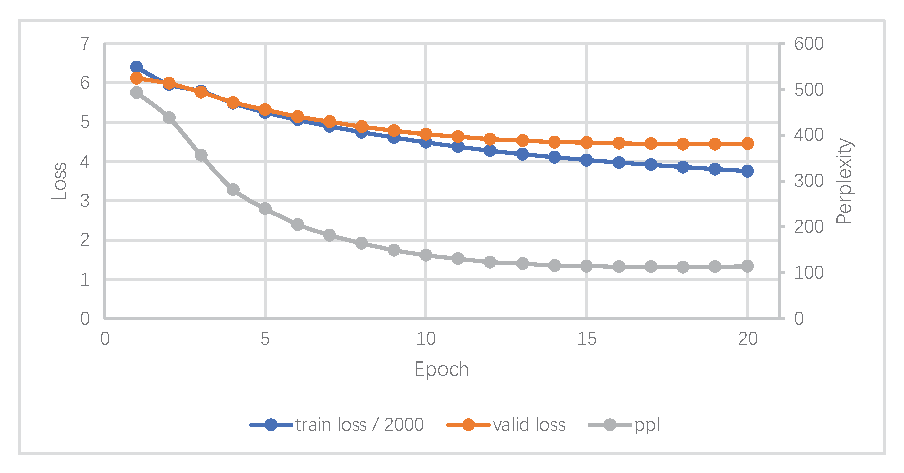
\includegraphics[scale=1]{lm_lstm.eps}
\caption{The training curve of the submitted LSTM model.}
\end{figure}

\begin{figure}[H]
\centering
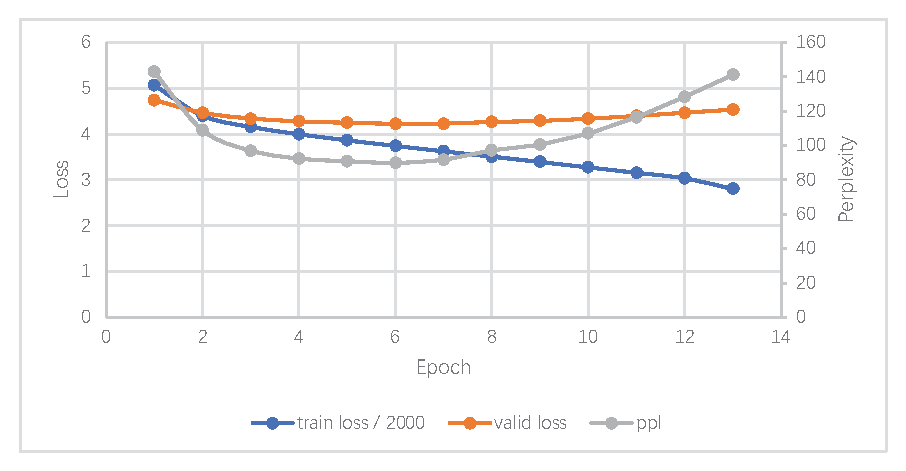
\includegraphics[scale=1]{lm_transformer.eps}
\caption{The training curve of the submitted Transformer model.}
\end{figure}

\subsection*{Generated samples}

\begin{figure}[H]
\centering
\includegraphics[scale=0.5]{lm_lstm_samples.png}
\caption{The generated samples of the submitted LSTM model.}
\end{figure}

\begin{figure}[H]
\centering
\includegraphics[scale=0.5]{lm_transformer_samples.png}
\caption{The generated samples of the submitted Transformer model.}
\end{figure}

\end{homeworkProblem}

\begin{homeworkProblem}[2 Classification]

\subsection*{\textcolor{red}{Requirements}}

\textcolor{red}{A custom vocabulary set is used so please copy \texttt{classification/vocab.txt} to \texttt{Datasets/CLS/vocab.txt}. Also, although the final submitted model do not use pre-trained Bert, please install \texttt{transformers}, since when initializing dataset, preprocessed-tokenized inputs are cached for quick retrieve afterwards. Two types of tokenized inputs are preprocessed: LSTM/Transformer style (using \texttt{dictionary.py} and \texttt{classification/vocab.txt}) for these two types of models, and Bert style (using tokenizer in \texttt{https://huggingface.co/bert-base-chinese/tree/main}) for pre-trained Bert model. The Bert tokenized inputs are never fed to models of LSTM or Transformer style.}

\subsection*{Implementation}

The overall structure comes from \cite{zhang2019dual}, in which an encoder $e(x)$ and a dual co-matching network $\textup{DCN}(P, Q, A)$ are involved. For each question, this model takes $P$ the passage, $Q$ the question and $\mathcal{A}=\{A_i\}$ the set of choices as inputs. There are many options for encoder $e(x)$, I implemented LSTM, Transformer and pre-trained Bert (Bert-base on Chinese corpus). Assume that $e(x)$ maps any input of length $L$ into a hidden feature of size $L \times h$ where $h$ is the hidden size.

First fix a choice $A_i$, then we calculate a feature matrix $C_i=[M^{pq};M^{pa_i};M^{qa_i}]$. Take $M^{pq}$ as example:
\begin{align}
    & H^p = e(P),\ H^q = e(Q); \\
    & G^{pq} = \textup{RowSoftMax}(H^p W (H^a)^{\top}),\ G^{qp} = \textup{ColumnSoftMax}(H^p W (H^a)^{\top}); \\
    & E^p = G^{pq} H^q,\ E^q = (G^{qp})^{\top} H^p; \\
    & S^p = \textup{ReLU}(E^p W_1^{pq}),\ S^q = \textup{ReLU}(E^q W_2^{pq}); \\
    & M^p = \textup{ColumnMax}(S^p),\ M^q = \textup{ColumnMax}(S^q); \\
    & g = \textup{Sigmoid}(M^p W_3^{pq} + M^q W_4^{pq} + b^{pq}); \\
    & M_{pq} = g M^p + (1 - g) M^q.
\end{align}
RowSoftMax takes softmax within each row, and ColumnSoftMax is similar; both of them maintains the shape of matrix. ColumnMax takes maximum within each column and returns a row vector. All $W_i^{pq}$'s and $b^{pq}$ are learnable.

Finally, the probability of choosing $A_i$ is
\begin{align}
    P(A_i|P,Q) = \frac{\exp(V^{\top} C_i)}{\sum_{j=1}^4 \exp(V^{\top} C_j)}.
\end{align}
$V$ is a vector of dimension $3h$ and is learnable.

\subsection*{Hyper-parameter tuning}

\begin{table}[H] 
  \begin{center}
    \begin{tabular}{|c|c|c|c|c|c|}
      \hline \textbf{Model type} & \textbf{Hidden size} & \textbf{\#Layers} & \textbf{\#Heads} & \textbf{Batch size} & \textbf{Accuracy ($\%$)}\\
      \hline \multirow{2}{*}{LSTM}        & 512                   & \multirow{2}{*}{2} & \multirow{2}{*}{-}  & $4 \times 1$ & \emph{\textbf{47.0}} \\
      \cline{2-2} \cline{5-6}             & 1024                  &                    &                     & $4 \times 4$ & 45.8 \\
      \hline \multirow{4}{*}{Transformer} & \multirow{4}{*}{512}  & \multirow{4}{*}{3} & \multirow{2}{*}{8}  & $1 \times 1$ & \textbf{46.0} \\
      \cline{5-6}                         &                       &                    &                     & $1 \times 4$ & 45.2 \\
      \cline{4-6}                         &                       &                    & \multirow{2}{*}{16} & $1 \times 1$ & 44.8 \\
      \cline{5-6}                         &                       &                    &                     & $1 \times 4$ & 44.5 \\
      \hline Bert                         & 768                   & -                  & -                   & $1 \times 4$ & \textbf{41.8} \\
      \hline
      
    \end{tabular}
    \caption{Hyper-parameters and corresponding (current) best accuracies on validation set. The boldface perplexities are the best. Italics are submitted. For batch size of $x \times y$, it means real batch size is $x$, and accumulating gradients over $y$ batches.}
    \label{classification_hyper}
  \end{center}
\end{table}

\subsection*{Discussion}

When training with pre-trained Bert, the lengths of passages (around 2000) may exceed the limit of Bert (512). My solution to this is to randomly take 4 (maybe overlapping) sections from the passage, each with length 500, and add their hidden features together as a surrogate for the whole passage.

Another problem brought about by the ultra-long passages is high memory consumption. The batch size cannot exceed $4$ on a 2080Ti and it drastically affects the training performance.

It can be seen from Table \ref{classification_hyper} that, Transformers and Bert are beaten by LSTMs. It is convincing that none of the models are adequately trained. The ultimate problem is that all the models are hard to train, especially the pre-trained Bert. Due to resource limitations, it is impossible for me to check every promising combination of hyper-parameters. One epoch for Bert takes around one hour, so experimenting consumes much time and computing power.

\end{homeworkProblem}

\bibliographystyle{plainnat}
\bibliography{ref}

% End edit to here
%%%%%%%%%%%%%%%%%%%%%%%%%%%%%%%%%%%%%%%%%%%%%%%%%%%%%%%%%%%%%

\end{spacing}
\end{document}

%%%%%%%%%%%%%%%%%%%%%%%%%%%%%%%%%%%%%%%%%%%%%%%%%%%%%%%%%%%%%
